\documentclass[a4paper,11pt]{article}

\usepackage{geometry}
\usepackage{listings}
\usepackage{mathrsfs}
\usepackage[font={small},labelfont={sf,bf}]{caption}
\usepackage{color}
\usepackage{amssymb}
\usepackage[utf8]{inputenc}
\usepackage{afterpage}
\usepackage[T1]{fontenc}
\usepackage{amsfonts}
\usepackage{mathtools}
\usepackage{amsmath}
\usepackage{verbatim}
\usepackage{bm}
\usepackage{bbm}
\usepackage{enumerate}
\usepackage{amsthm}
\usepackage{stmaryrd}

\geometry{a4paper,top=3cm,bottom=3cm,left=2cm,right=2cm,heightrounded, bindingoffset=5mm}

\theoremstyle{definition}
\newtheorem{definition}{Definition}[section]
\theoremstyle{plain}
\newtheorem{theo}[definition]{Theorem}
\newtheorem{prop}[definition]{Proposition}
\newtheorem{lemma}[definition]{Lemma}
\newtheorem{cor}[definition]{Corollary}
\newtheorem{ex}[definition]{Example}
\theoremstyle{remark}
\newtheorem{rem}[definition]{Remark}
\newtheorem{rem*}[definition]{}

\newcommand*\mcup{\mathbin{\mathpalette\mcupinn\relax}}
\newcommand*\mcupinn[2]{\vcenter{\hbox{$\mathsurround=0pt
  \ifx\displaystyle#1\textstyle\else#1\fi\bigcup$}}}
\newcommand*\mcap{\mathbin{\mathpalette\mcapinn\relax}}
\newcommand*\mcapinn[2]{\vcenter{\hbox{$\mathsurround=0pt
  \ifx\displaystyle#1\textstyle\else#1\fi\bigcap$}}}
\DeclarePairedDelimiter{\abs}{\lvert}{\rvert}
\DeclarePairedDelimiter{\norm}{\lVert}{\rVert}
\DeclarePairedDelimiter{\parr}{(}{)}
\DeclarePairedDelimiter{\parq}{[}{]}
\DeclarePairedDelimiter{\parqq}{\llbracket}{\rrbracket}
\DeclarePairedDelimiter{\bra}{\lbrace}{\rbrace}
\DeclarePairedDelimiter{\ceil}{\lceil}{\rceil}
\DeclarePairedDelimiter{\prodscal}{\langle}{\rangle}
\DeclarePairedDelimiter{\floor}{\lfloor}{\rfloor}
\DeclareMathOperator*{\argmin}{arg\,min}
\DeclareMathOperator*{\argmax}{arg\,max}
\DeclareMathOperator*{\expval}{\mathbb{E}}
\DeclareMathOperator*{\varval}{\mathrm{Var}}

\begin{document}

\title{Applied Stochastic Analysis \\ Homework assignment 4}
\author{Luca Venturi}
\maketitle

\section*{Exercise 1}

\paragraph*{(a)} Calculating its eigenvalues/vectors, $Q$ can be decomposed as 
$$
Q = \parr*{\begin{array}{cc}
1 & \mu \\ 1 & -\lambda
\end{array}}\parr*{\begin{array}{cc}
0 & 0 \\ 0 & -\lambda-\mu
\end{array}}\parr*{\begin{array}{cc}
\lambda/(\lambda+\mu) & \mu/(\lambda+\mu) \\ 1/(\lambda+\mu) & -1/(\lambda+\mu)
\end{array}}.
$$
Therefore the transition probabilities matrix is given by
\begin{align*}
P(t) & = e^{tQ} = \parr*{\begin{array}{cc}
1 & \mu \\ 1 & -\lambda
\end{array}}\parr*{\begin{array}{cc}
1 & 0 \\ 0 & e^{-(\lambda+\mu)t}
\end{array}}\parr*{\begin{array}{cc}
\lambda/(\lambda+\mu) & \mu/(\lambda+\mu) \\ 1/(\lambda+\mu) & -1/(\lambda+\mu)
\end{array}} \\ & = \frac{1}{\lambda+\mu}\parr*{\begin{array}{cc}
\lambda + \mu e^{-(\lambda+\mu)t} & \mu-\mu e^{-(\lambda+\mu)t} \\
\lambda-\lambda e^{-(\lambda+\mu)t} & \mu+\lambda e^{-(\lambda+\mu)t}
\end{array}}.
\end{align*}

\paragraph*{(b)} The stationary distribution is given by
$$
\pi = \parr*{\begin{array}{cc} \frac{\lambda}{\lambda+\mu} & \frac{\mu}{\lambda+\mu} \end{array}}.
$$
Moreover, since $\lambda+\mu>0$, for $t\to+\infty$ we have $e^{-(\lambda+\mu)t}\to 0$ and thus
$$
P(t) \to \frac{1}{\lambda+\mu}\parr*{\begin{array}{cc}
\lambda & \mu \\ \lambda & \mu
\end{array}} = \begin{bmatrix}
\pi \\ \pi
\end{bmatrix}.
$$

\paragraph*{(c)} Thanks to previous part, as $t\to+\infty$ it holds that
$$
\expval\parq{X(t)^2\,|\,X(0)=1} = 1\cdot p_{11}(t) + 4\cdot p_{12}(t) \to \frac{\lambda+4\mu}{\lambda+\mu}
$$
and
$$
\expval\parq{X(t)^2\,|\,X(0)=2} = 1\cdot p_{21}(t) + 4\cdot p_{22}(t) \to \frac{\lambda+4\mu}{\lambda+\mu}.
$$
Clearly, the value above is exactly the $2$-nd moment of the distribution $\pi$.

\section*{Exercise 2}

Consider
$$
P = \parr*{\begin{array}{cc} \alpha & 1-\alpha \\ 1-\alpha & \alpha
\end{array}}
$$
for $0<\alpha<1$. If there exists a ctMC with transition probabilities $P(t)$ such that $P(1)=P$, then $P(t)$ must have the form
$$
P(t) = e^{tQ}.
$$ 
Now the above equation implies that $\mathrm{det}(P(t))>0$ for every $t\geq0$. Indeed it must be $\mathrm{det}(P(t))\neq0$ since $P(t)$ has inverse $P(t)^{-1}=e^{-tQ}$ and it must also be $\mathrm{det}(P(t))\geq0$ since 
$$
\mathrm{det}(P(t))= \mathrm{det}\parr{P\parr{t/2}^2} = \mathrm{det}\parr*{P\parr*{t/2}}^2\geq0.
$$
So if the dtMC with transition matrix $P$ can be embedded in a ctMC, it must hold
$$
2\alpha -1 = \det(P) = \det(P(1)) > 0,
$$
i.e. $\alpha\in(\frac{1}{2},1)$. On the other hand, if $\alpha\in(\frac{1}{2},1)$ then one can take 
\begin{align*}
P(t) & = \parr*{\begin{array}{cc}
1 & 1 \\ 1 & -1
\end{array}}\parr*{\begin{array}{cc}
1 & 0 \\ 0 & (2\alpha-1)^t
\end{array}}\parr*{\begin{array}{cc}
1/2 & 1/2 \\ 1/2 & -1/2
\end{array}} \\ & = \parr*{\begin{array}{cc}
1/2 + 1/2\cdot(2\alpha-1)^t & 1/2 - 1/2\cdot(2\alpha-1)^t \\ 
1/2-1/2\cdot(2\alpha-1)^t & 1/2 + 1/2\cdot(2\alpha-1)^t
\end{array}},
\end{align*}
for $t\geq 0 $, i.e. the dtMC with transition matrix $P$ can be embedded in a ctMC with transition probabilities $P(t)$ such that $P(1)=P$.

\section*{Exercise 3}

We have that
\begin{align*}
\sum_i\pi_iP\bra{Y_1=j\,|\,Y_0=i} & = \sum_i\pi_iP\bra{X_{T_1}=j\,|\,X_0=i} \\ & = \sum_i\pi_i\int_0^{+\infty}P\bra{X_{T_1}=j\,|\,X_0=i, T_1=t}\,dP_{T_1}(t) \\ & = \sum_i\pi_i\int_0^{+\infty}P\bra{X_t=j\,|\,X_0=i, T_1=t}\,dP_{T_1}(t) \\ & = \sum_i\pi_i\int_0^{+\infty}P\bra{X_t=j\,|\,X_0=i}\,dP_{T_1}(t) \\ & = \int_0^{+\infty}\sum_i\pi_iP\bra{X_t=j\,|\,X_0=i}\,dP_{T_1}(t) = \int_0^{+\infty}\pi_j\,dP_{T_1}(t) = \pi_j,
\end{align*}
i.e., $\pi$ is a stationary distribution for $Y$ too.

\section*{Exercise 4}

If $T_n$ is the time of the $n$-th arrival of $X$, where $X=\bra{X_t}_{t\geq0}\sim\mathrm{Poi}(\lambda)$, then what we want to show is that 
\begin{equation}\label{ex4}
P\bra{T_1\leq s\,|\,T_2>t,\,T_1\leq t} = \frac{s}{t}
\end{equation}
for $s\in[0,t]$. If we consider $S_n=T_n-T_{n-1}$ for $n>1$, $S_1=T_1$, it holds that the $\bra{S_n}_{n\geq1}$ are independent and have distribution $\mathrm{exp}(\lambda)$. Note that we can rewrite the lhs of (\ref{ex4}) as
\begin{equation}\label{ex4.1}
P\bra{T_1\leq s\,|\,T_2>t,\,T_1\leq t} = P\bra{S_1\leq s\,|\,S_1+S_2>t,\,S_1\leq t} = \frac{P\bra{S_1\leq s,\,S_1+S_2>t}}{P\bra{S_1\leq t,\,S_1+S_2>t}}.
\end{equation}
Now if $s,t\geq 0$ we have that
$$
P\bra{S_1\leq s,\,S_1+S_2>t} = \int_A \lambda^2e^{-\lambda(x+y)}\,dxdy,
$$
where $A=\bra{(x,y)\in[0,+\infty)\,:\,x\leq s,\,x+y>t}$. Applying the change of variables $u=x,v=x+y$, the above becomes
$$
P\bra{S_1\leq s,\,S_1+S_2>t} = \int_0^s\int_t^{+\infty} \lambda^2e^{-\lambda v}\,dudv = s\lambda e^{-\lambda t}.
$$
Therefore (\ref{ex4.1}) gives
$$
P\bra{T_1\leq s\,|\,T_2>t,\,T_1\leq t} = \frac{s\lambda e^{-\lambda t}}{t\lambda e^{-\lambda t}} = \frac{s}{t},
$$
which is exactly (\ref{ex4}), i.e., what we wanted to prove.

\section*{Exercise 5}

\paragraph*{(a)}

If $t>0$, $i,j\in S$, we have that
\begin{align*}
\abs{p_{ij}(t+h)-p_{ij}(t)} & = \abs*{\sum_kp_{ik}(h)p_{kj}(t)-p_{ij}(t)} \leq p_{ij}(t)(1-p_{ii}(h)) + \sum_{k\neq i}p_{ik}(h)p_{kj}(t) \\ & \leq (1-p_{ii}(h)) + \sum_{k\neq i}p_{ik}(h) = 2(1-p_{ii}(h)) \to 0,
\end{align*}
as $h\to0$ (to take into account $h<0$ one can simply define $p_{ij}(t)$ for $t\in\mathbb{R}$ as an even function).

\paragraph*{(b)} 

Since $p_{ij}(t)\in(0,1)$ for every $i,j\in S$ and $t\in(0,1)\geq 0$ and $t\mapsto -\log t$ is a decreasing function for $t\in(0,1)$, we have
\begin{align*}
g(t+s) & = -\log p_{ii}(t+s) = -\log \sum_kp_{ik}(t)p_{ki}(s) \leq -\log p_{ii}(t)p_{ii}(s) \\ & = -\log p_{ii}(t)-\log p_{ii}(s) = g(t)+g(s).
\end{align*}

\paragraph*{(c)}

By the previous part we know that
$$
\lim_{t\to0^+}\frac{\log p_{ii}(t)}{t} = \inf_{t>0}\frac{\log p_{ii}(t)}{t} = \lambda \in [-\infty,0].
$$
Thanks to this and to the fact that $p_{ii}(t)\to 1$ as $t\to0^+$, it holds that
$$
q_{ii}=\lim_{t\to0^+}\frac{p_{ii}(t)-1}{t} = \lim_{t\to0^+}\frac{p_{ii}(t)-1}{\log p_{ii}(t)}\cdot\frac{\log p_{ii}(t)}{t} = \lim_{x\to1}\frac{x-1}{\log x}\cdot\lim_{t\to0^+}\frac{\log p_{ii}(t)}{t} = 1\cdot\lambda = \lambda  \in [-\infty,0].
$$

\section*{Exercise 6}

In the attached paper there is the \texttt{python} script. The matrix $Q$ is obtained by considering the adjacency matrix $E$ of the graph induced by the chessboard and replacing the diagonal with minus the sum of the entries of the corresponding rows. The matrix $P$ is obtained by $E$ by normalizing its rows so that they sum to 1 and $\lambda$ is the vector of minus the diagonal entries of $Q$. The value of the mean first passage time obtained using backward Kolmogorov equations is $\mathrm{mfpt}_a\simeq 14.857$. We can find almost the same value using Kinetic Monte Carlo, but this method requires an high number of iterations (I used $N=2^{16}$) to converge and even for such a number of iteration (i.e. $N=2^{16}$) it's not too much reliable. 
\begin{figure}[htbp]
\centering
\begin{minipage}[c]{.47\textwidth}
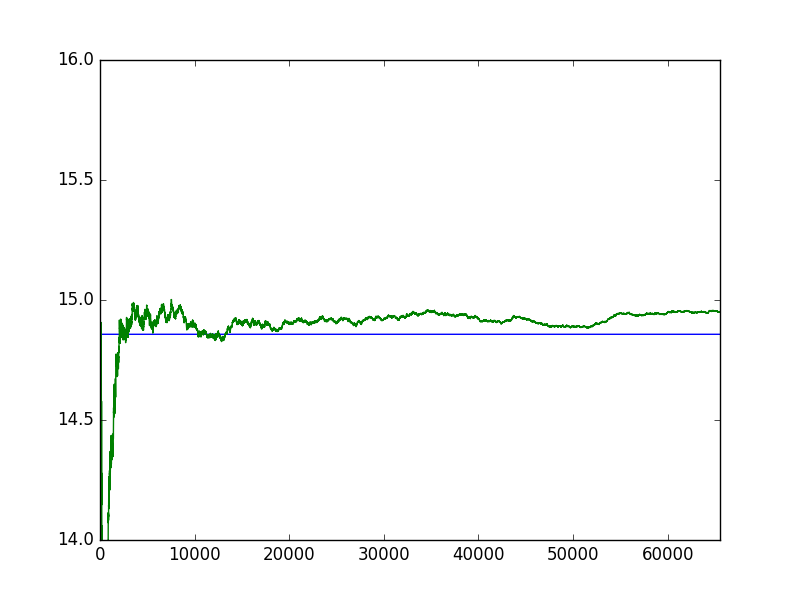
\includegraphics[width=\textwidth,
keepaspectratio]{ex4.png}
\end{minipage}
\hspace{4mm}
\begin{minipage}[c]{.47\textwidth}
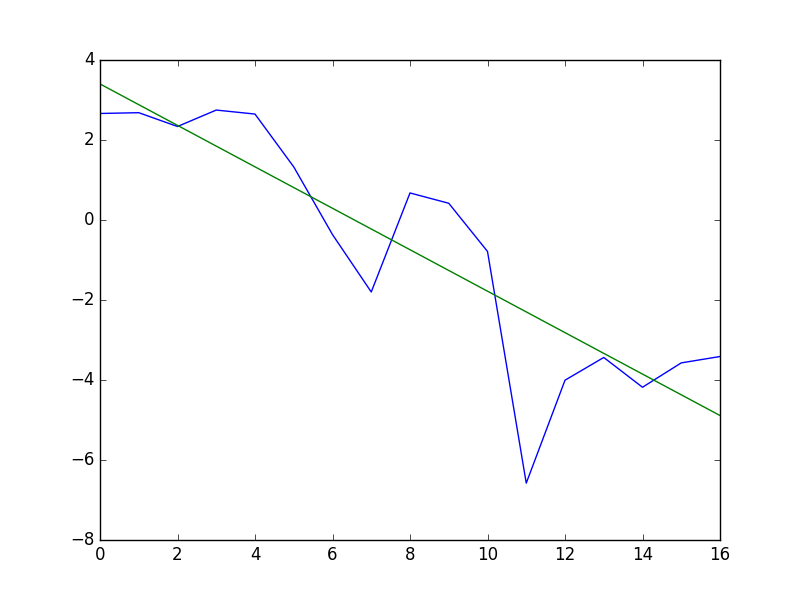
\includegraphics[width=\textwidth,
keepaspectratio]{ex4_1.png}
\end{minipage}
\caption{ \label{figure:ex6}}
\end{figure}
In the left figure in Figure \ref{figure:ex6} we plot the value $\mathrm{mfpt}_b$ as a function of $N$ against the 'real' value $\mathrm{mfpt}_a$. In the right figure in Figure \ref{figure:ex6} we plot the value of error $\log_2\abs{\mathrm{mfpt}_b-\mathrm{mfpt}_a}$ for $N=2^k, k=0,\dots,16$. According to part (c), this should go approximately as a line, so we plot it against its linear regression. The linear regression gives an estimate of $\alpha\simeq 0.51$ (this is the value of $\alpha$ I obtained when I run the script who gave the figures in Figure \ref{figure:ex6} this value slightly changes every time we run the script). I think this value could be justified in the following way. If $\expval\parq{T}$ is the value of the mean first passage time and $Y_N = N^{-1}\sum_{k=1}^NT_k$ is our average approximation obtained generating $N$ trajectories, then by Chebyshev inequality we have
$$
P\bra{\abs{Y_N-\expval\parq{T}}>\varepsilon} \leq \frac{\varval(T)}{N\varepsilon^2},
$$
for any $\varepsilon\in(0,1)$, which implies that with probability at least $1-\varepsilon$, the Monte Carlo average $Y_N$ lies within
$(\varval(T)/(N\varepsilon))^{1/2}$ of the true expected value  (i.e. $\alpha=0.5$).

\end{document}